\documentclass{beamer}
\usetheme{Madrid}
\setbeamercovered{invisible}
\setbeamertemplate{navigation symbols}{}
%
\usepackage{tabularx}
\usepackage{graphicx}
\usepackage{algorithm}
\usepackage[noend]{algpseudocode}
\usepackage{beamerthemesplit}

\graphicspath{{../images/}}

%
\title[Florida International University]{SSD-based Energy Efficient Cloud Storage}
\author{Salma Rodriguez}
\institute[University] {
Florida International University \\
\medskip
{\emph{srodr063@fiu.edu}}}
\date{\today}
%
\begin{document}
%
\section{Introduction}
%
\begin{frame}
\titlepage
\end{frame}
%
\begin{frame}
\frametitle{Motivation}
\begin{block}
{Solid State Technology}
High capacity EEPROM devices
reduces energy consumption when they are used
as cache for data on a storage server
\end{block}
\begin{block}
{Distributed SSD Caching}
With a distributed caching solution, the working set of user
applications is kept mostly in flash memory.
\end{block}
\begin{block}
We explore the properties of dynamic spin control of storage
server disks and replication of cold pages.
\end{block}
\end{frame}
%
\begin{frame}
\frametitle{Linux Device Mapper}
\begin{tabular}{p{0.463\linewidth}|p{0.463\linewidth}}
\hline
\begin{itemize}
 \item pseudo device is the only device visible to applications
 \item device mapper facilitates mapping between two block devices
 \item kernel module uses device mapper to map bios from pseudo device
\end{itemize} &
\begin{figure}
 %\caption{Device Mapper Layout}
 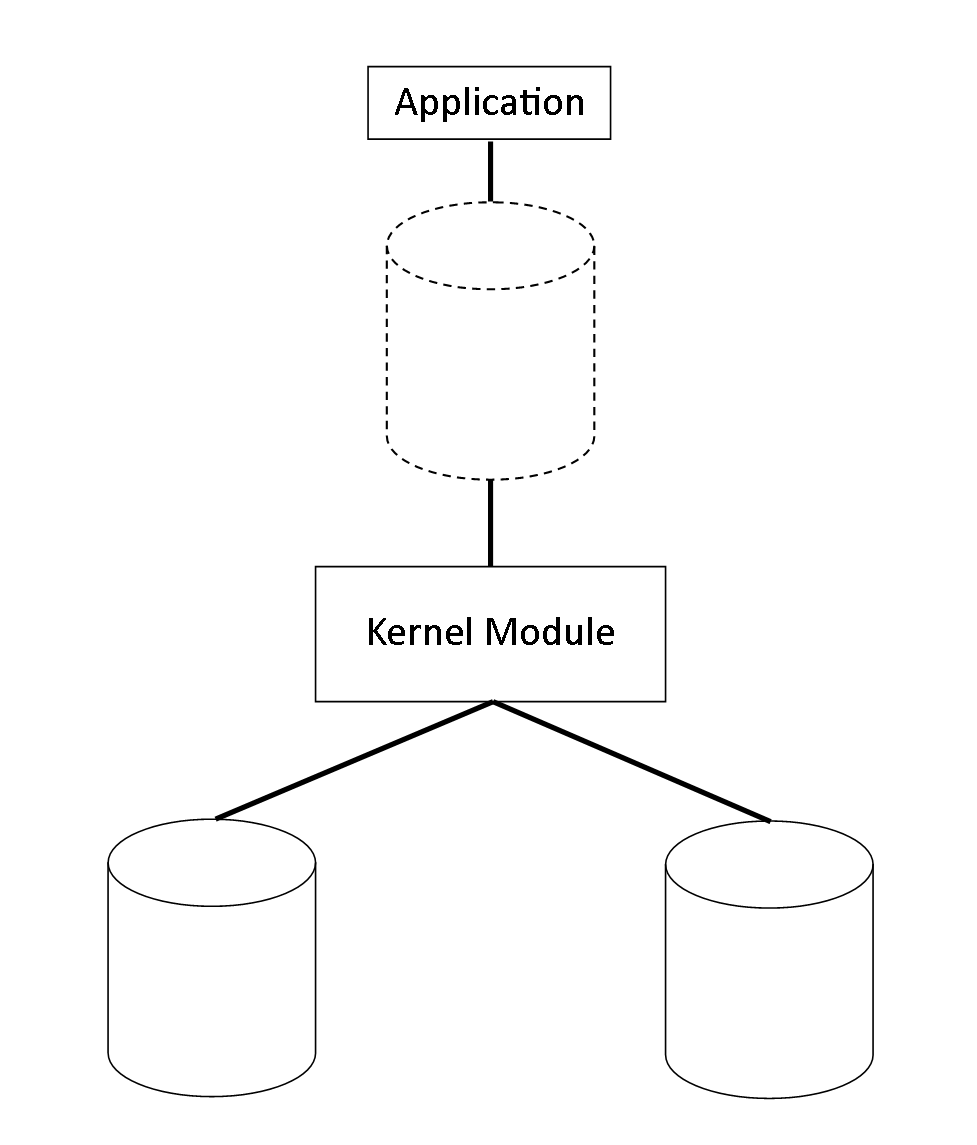
\includegraphics[scale=.30]{DMC.png}
 \label{fig:dmc}
\end{figure} \\
\hline
\end{tabular}
\end{frame}
%
\begin{frame}
\frametitle{Device Mapper Cache}
% \begin{figure}
\end{frame}
%
\section{Dynamic Disk Spin}
%\Let{$k$}{current time in seconds}
%\Let{$c$}{time since last cache miss}
\begin{frame}
% \begin{algorithm}
\frametitle{Disk Spin: Implementation}
\bf Algorithm 1 \rm Spinning the disk up or down dynamically
%\caption{Algorithm for dynamic spinning the disk up or down
%\label{alg:dyn-spinning}}
\begin{algorithmic}[1]
\Procedure{Spin Up or Down}{}
\While {true}
 \If{disk is spinning}
  \State $k\gets$ current time in seconds
  \State $c\gets$ time since last cache miss
  \If{$c$ + $20 \leq k$}
   \State spin down the disk and change state to not spinning
  \EndIf
 \Else \Comment{disk is not spinning}
  \If{DM Cache is blocking on a cache miss}
   \State spin up the disk and change state to spinning
   \State unblock DM Cache
  \EndIf
 \EndIf
\EndWhile
\EndProcedure
\end{algorithmic}
% \end{algorithm}
\end{frame}
%
\section{Replication}
\begin{frame}
\frametitle{Consistent Hashing}
Idea: replicate data evenly with as little disruption
as possible when nodes join and exit a network. \\
\begin{theorem}
For any set of N nodes and K keys, with high probability:
\newline\newline
1. Each node is responsible for at most (1 + $\epsilon$)K/N keys
\newline\newline
2. When an (N + 1)st node joins or leaves the network,
   responsibility for O(K/N) keys changes hands (to or from
   the joining or leaving node)
\end{theorem}
Here $\epsilon$ may vary but has an upper bound of \textit{O(log N)}.
\end{frame}
%
%section{Verbatim}
%begin{frame}[fragile]
%frametitle{Verbatim}
%begin{example}[Putting Verbatim]
%begin{verbatim}
%begin{frame}
%frametitle{Outline}
%begin{block}
%Why Beamer?}
%
%end{block}
%
%end{frame}\end{verbatim}
%end{example}
%end{frame}
%
%begin{frame}[fragile]
%
%xample of the \verb|\cite| command to give a reference:
%xample of citation using \cite{key1} follows on.
%end{frame}
%
\section{References}
\begin{frame}
\frametitle{References}
\footnotesize {
\begin{thebibliography}{99}
 \bibitem[Label1, 2010]{key1} Author's name (1987)
 \newblock Title of the paper.
 \newblock \emph{Journal Name} 55(4), 765 -- 799.
\end{thebibliography}
}
\end{frame}
%
\end{document}
